% Working manuscript, revised 2026-10-07. Original: 20261007/original/.
% ASIACCS 2027: standard ACM two-column layout, no font/margin overrides.
% DOI, ISBN, submission ID and anonymous artifact URL remain unassigned.
\documentclass[sigconf,anonymous,pbalance]{acmart}
\usepackage{amsmath}
\usepackage{booktabs}
\usepackage{siunitx}
\usepackage{tikz}
\usetikzlibrary{arrows.meta,positioning}
\sisetup{group-separator={,},group-minimum-digits=4,group-digits=integer,detect-all}
\setcopyright{acmlicensed}
\copyrightyear{2027}
\acmYear{2027}
\acmDOI{}
\acmISBN{}
\acmConference[ASIACCS '27]{ACM Asia Conference on Computer and Communications Security}{July 12--16, 2027}{Macau}
\IfFileExists{tables/quality.tex}{\newcommand{\paperassetroot}{.}}{\newcommand{\paperassetroot}{20261007}}
\newcommand{\globalidx}{\mathrm{G}}
\newcommand{\ctx}{\mathcal{C}}

\begin{document}
\title{TAILGUARD: Selective Context Experts for Long-Tailed Intrusion Detection}
\author{Anonymous}

\begin{abstract}
An intrusion detector must use newly available attack examples while retaining its ability to distinguish existing attacks from benign traffic. A static aggregate classification score provides only part of the evidence needed to assess this capability. We investigate TabPFN as a basis for updating a detector through its labelled context and for specializing prediction on under-represented attacks. Our current design combines a Global context with a bank of context experts, a scorer that decides whether to invoke an expert, and a verifier that decides whether to adopt its prediction. Experts share a pretrained backbone and differ in their contexts: a common anchor is combined with examples selected from clusters of Global residual information. We report exploratory evidence on conflict-filtered CIC2018 and ToN-IoT, including current tabular baselines, expert intervention statistics, and a separate comparison of context expansion with XGBoost refitting. Results show a substantial Scanning improvement on ToN-IoT, but no selected expert intervention on CIC2018 and no consistent advantage on the rarest attacks. Context expansion also does not establish an overall cost advantage over XGBoost under the measured workload. These observations motivate evaluating specialization and intervention jointly, with attack-wise performance, benign false alarms, and measured update and inference costs.
\end{abstract}

\begin{CCSXML}
<ccs2012>
 <concept>
  <concept_id>10002978.10003001.10003002</concept_id>
  <concept_desc>Security and privacy~Intrusion detection systems</concept_desc>
  <concept_significance>500</concept_significance>
 </concept>
 <concept>
  <concept_id>10010147.10010257.10010258.10010259</concept_id>
  <concept_desc>Computing methodologies~Supervised learning by classification</concept_desc>
  <concept_significance>300</concept_significance>
 </concept>
</ccs2012>
\end{CCSXML}
\ccsdesc[500]{Security and privacy~Intrusion detection systems}
\ccsdesc[300]{Computing methodologies~Supervised learning by classification}
\keywords{intrusion detection, long-tailed classification, tabular foundation models, in-context learning, selective expert activation}
\maketitle

\noindent\textit{Working draft, 7 October 2026.} The architecture and evaluation remain under development. Reported results are existing single-seed observations; pending evaluations are identified explicitly.

\section{Introduction}
\label{sec:intro}
Newly labelled attacks create a practical question for an intrusion detector: how should the detector incorporate these examples without unnecessarily disrupting decisions on benign traffic and previously observed attacks? A classifier trained once on all available attack labels does not directly evaluate this update process. The issue is particularly relevant when attack classes have very different frequencies. Improving an average score can leave rare attacks undetected or increase the number of benign flows incorrectly labelled as attacks.

Our inputs are tabular flow records. We use XGBoost as a strong supervised baseline~\cite{chen2016xgboost}. A different mechanism is offered by TabPFN: a pretrained predictor conditions on a labelled context~\cite{hollmann2023tabpfn,hollmann2025tabpfn}. With a frozen backbone, replacing or extending that context changes the prediction task without optimizing the backbone on each target dataset. The operational question is whether this mechanism yields useful attack detection and retention at an acceptable update and inference cost. The absence of backbone retraining alone is insufficient evidence of such an advantage.

Our research goal is to improve detection of under-represented attacks through the use of available labelled examples. Context composition is central to this goal because the examples presented to the predictor may be a limited subset of a much larger training pool. A single Global context must represent benign traffic and multiple attack families simultaneously. Additional contexts can emphasize Global error patterns, but emphasizing an attack may also cause an expert to predict it for benign flows or other attacks. Expert specialization therefore needs both a construction rule and a mechanism for deciding when its output is useful.

TAILGUARD investigates this combination. The current implementation constructs context experts from a shared anchor and residual-based blocks, using one frozen TabPFN backbone. A scorer evaluates candidate experts before expert inference; a verifier then assesses the selected expert's prediction before replacing the Global output. Expert construction, activation, and output adoption are separate decisions. We describe the implemented configuration without assuming that its present context recipe or selection objectives are final.

The current evidence has two distinct roles. Static comparisons on conflict-filtered CIC2018 and ToN-IoT characterize the context-expert system against tabular baselines. A separate experiment introducing attack classes compares a single TabPFN with a refitted XGBoost on identical cumulative examples. That experiment motivates the update question but does not evaluate an updating expert bank. The present system improves some ToN-IoT attacks, especially Scanning, while the CIC2018 policy retains Global predictions throughout. These mixed outcomes make it necessary to assess which corrections transfer to an executable selection policy rather than treating the existence of a correct expert prediction as a deployed result.

\paragraph{Scope and contributions of this draft.}
We present (i) a context-expert design that separates residual-based specialization from query-time activation and adoption; (ii) an evaluation that distinguishes expert predictions, policy decisions, and changes to Global correctness; and (iii) exploratory static and update comparisons that report attack-wise outcomes together with data access and computational cost. We do not claim a universal performance advantage, a demonstrated online speedup, or detection of attacks for which no labelled examples are available. Those claims require additional evidence.

\section{Related Work}
\label{sec:related}
We organize related work around task-specific tabular learning, tabular foundation models, context and posterior adaptation, and expert specialization.

\subsection{Task-Specific Tabular Learning}
XGBoost~\cite{chen2016xgboost} constructs a supervised tree ensemble through gradient boosting. In our study it represents a detector whose fitted parameters are updated from the available labelled examples. We evaluate both a matched training-subset baseline and a full-training-pool baseline. The former controls example access against the Global context, whereas the latter measures the benefit of allowing the tree model to use the larger pool.

\paragraph{Discussion.}
A static tree-model result does not by itself answer how the model behaves when the set of available attack labels expands. Our response is to compare explicit update procedures on identical cumulative examples and to investigate context changes as an alternative way of incorporating information. The chosen comparator is full XGBoost refitting; this is an experimental choice, not a claim that all tree-based updates require full retraining. New-attack performance, existing-class retention, benign false alarms, and both update and inference time must support any advantage attributed to context-based updating.

\subsection{Tabular Foundation Models}
TabPFN learns a prediction procedure through pretraining on synthetic tabular tasks and applies it to new datasets using in-context learning~\cite{hollmann2023tabpfn}. Subsequent work demonstrates strong performance on small tabular datasets and develops a more capable tabular foundation model~\cite{hollmann2025tabpfn}. These studies motivate using a pretrained predictor as a reusable component. Section~\ref{sec:tabpfn} defines the interface needed here; the exact checkpoint used in our experiments is specified separately from these foundational papers.

\paragraph{Discussion.}
Strong general tabular performance does not determine which labelled examples should represent an imbalanced IDS dataset, nor whether changing that representation improves rare-attack detection without increasing false alarms. We investigate a Global context together with specialized contexts instead of assuming that one context is adequate for every query. The relevant evidence is the gain of the complete context-and-selection system over the same Global predictor, including cases where specialization introduces new errors. This is a problem addressed by our design, not a guarantee supplied by pretraining.

\subsection{Context and Posterior Adaptation}
\paragraph{BoostPFN.}
BoostPFN~\cite{wang2025boostpfn} treats PFNs as weak learners to extend their use to larger datasets through boosting. It is a direct comparison for exploiting a training pool through multiple smaller PFN contexts rather than placing the entire pool in one model input.

\paragraph{Discussion.}
The distinction we investigate is how multiple predictions are used: our experts offer candidate corrections to a retained Global decision, with a query-specific activation and adoption policy. This differs from using boosting to build an aggregate predictor. Whether that distinction improves attack-wise precision and recall is empirical; it must be tested at stated data and compute budgets, without treating BoostPFN's general scaling objective as a demonstrated weakness on IDS data.

\paragraph{LoCalPFN.}
LoCalPFN~\cite{thomas2024retrieval} combines nearest-neighbour context retrieval with task-specific fine-tuning. It adapts the predictor to local subsets and directly addresses the limitations of a single context for larger and more complex tabular tasks. Our evaluated LoCalPFN baseline includes its fine-tuning stage.

\paragraph{Discussion.}
Local relevance and predicted corrective value are different criteria. Our current approach constructs a reusable context bank from Global residual information, then estimates whether a bank member should intervene on a query. It retains a frozen TabPFN backbone in the proposed configuration. We must therefore compare the effect of context specialization and selection while reporting LoCalPFN's fine-tuning and retrieval costs explicitly. Neither feature proximity nor residual membership is assumed to guarantee superior classification.

\paragraph{DistPFN.}
DistPFN~\cite{lee2026distpfn} adjusts test-time class probabilities using the context class prior and aggregated model predictions to address label shift, without additional model training. We evaluate its posterior adjustment on the stored Global TabPFN-v3 probabilities, rather than replacing the Global context.

\paragraph{Discussion.}
Posterior adjustment addresses class-prior effects; our proposed mechanism changes the labelled examples available to a candidate predictor and controls when its output is adopted. The comparison asks whether this additional mechanism yields useful corrections beyond prior adjustment. Our DistPFN implementation uses aggregate predictions over the unlabelled test batch, which is disclosed as batch-level information access. Its cost includes the Global computation, and its protocol should not be presented as a strictly causal streaming method.

\subsection{Long-Tailed Expert Specialization}
RIDE~\cite{wang2020long} combines multiple distribution-aware experts with a diversity objective and dynamic routing for long-tailed recognition. It provides a relevant precedent for using expertise and conditional computation to address class imbalance. Its learned expert construction is distinct from changing the labelled context supplied to a shared pretrained tabular predictor.

\paragraph{Discussion.}
Our design specializes through context composition and learns intervention decisions relative to a Global reference. This raises a specific question: can a context expert correct difficult attacks while avoiding erroneous replacements on other classes? We evaluate raw expert predictions on common populations and the corrections actually retained by the selection policy. The existence of experts, or a favourable label-assisted assignment, is insufficient to establish this property. We do not claim novelty from the generic use of experts or routing alone.

\section{Preliminaries}
\label{sec:prelim}
\subsection{Long-Tailed Classification}
Let $\mathcal{D}=\{(x_i,y_i)\}_{i=1}^{N}$ contain tabular inputs $x_i\in\mathbb{R}^{d}$ and labels in $\mathcal{Y}=\{1,\ldots,C\}$. Class counts $n_c$ may differ substantially; the imbalance ratio is $\max_c n_c/\min_c n_c$ over nonempty classes. We use \emph{tail} descriptively for classes with small support in the fixed evaluation population and report that support explicitly. The number of examples selected into a context is a separate quantity. A rare class need not be difficult, and a difficult class need not be the rarest.

For each class, precision measures the correctness of predictions assigned to that class, while recall measures coverage of its true examples. F1 combines the two; macro-F1 gives equal weight to the included classes. A class can attain high recall by attracting many predictions and still have low F1 because of false positives. Benign false-alarm rate is the fraction of true benign examples predicted as attacks. These quantities must be interpreted together.

\subsection{TabPFN and In-Context Learning}
\label{sec:tabpfn}
A TabPFN prediction is conditioned on a labelled context $\ctx=\{(x_j,y_j)\}_{j=1}^{m}$ and an unlabelled query $x$~\cite{hollmann2023tabpfn,hollmann2025tabpfn}:
\begin{equation}
 p_{\theta}(y\mid x,\ctx),\qquad
 \hat y=\arg\max_{c\in\mathcal{Y}}p_{\theta}(c\mid x,\ctx).
 \label{eq:icl}
\end{equation}
In frozen-backbone use, $\theta$ is held fixed across target tasks. The labels in $\ctx$ belong to context examples; the query's true label is not supplied. Changing $\ctx$ changes the conditioning information even when $\theta$ is unchanged. Implementation work such as preprocessing and cache construction may still be required when a context is updated. Fine-tuning is a different mode of use and is stated explicitly when a baseline employs it.

\subsection{Experts and Conditional Computation}
An expert ensemble contains predictors $f_1,\ldots,f_K$ whose information or specialization may differ. Mixture-of-experts models use input-dependent mechanisms to select or combine expert outputs~\cite{jacobs1991adaptive}. Here we require only the general distinction between the expert bank and the rule for using that bank. An activation mechanism may select a subset of experts; an output decision may subsequently retain a reference prediction or use an expert prediction. Experts need not own disjoint classes, and activation does not necessarily imply adoption. The construction and decision rules specific to our system are introduced in Section~\ref{sec:approach}.

\section{Proposed Approach}
\label{sec:approach}
\subsection{Objective and Information Flow}
We seek corrections to a Global classifier that improve under-represented attack detection while controlling damage to existing decisions. Define $p_{\globalidx}(x)=p_{\theta}(\cdot\mid x,\ctx_0)$ and $p_k(x)=p_{\theta}(\cdot\mid x,\ctx_k)$ for the Global context and expert contexts. The Global and experts use the same pretrained backbone; specialization is implemented through their contexts. Separate lightweight models learn the scorer and verifier functions. Figure~\ref{fig:architecture} distinguishes their roles.

\begin{figure*}[t]
\centering
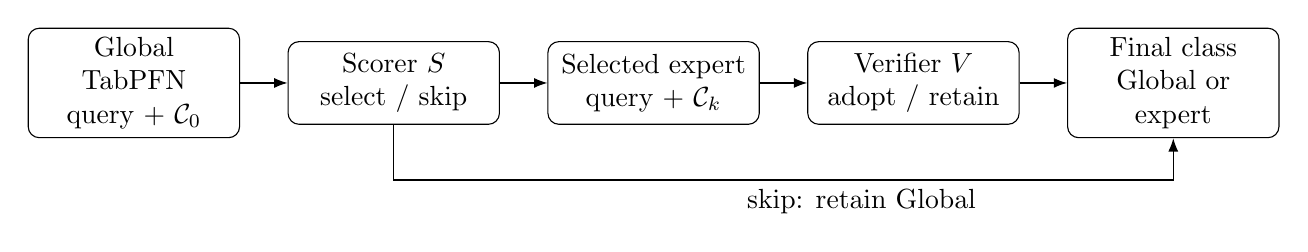
\begin{tikzpicture}[box/.style={draw,rounded corners,align=center,text width=2.45cm,minimum height=1.05cm},>=Latex]
\node[box] (g) at (0,0) {Global TabPFN\\query + $\ctx_0$};
\node[box] (s) at (3.3,0) {Scorer $S$\\select / skip};
\node[box] (e) at (6.6,0) {Selected expert\\query + $\ctx_k$};
\node[box] (v) at (9.9,0) {Verifier $V$\\adopt / retain};
\node[box] (o) at (13.2,0) {Final class\\Global or expert};
\draw[->] (g) -- (s);
\draw[->] (s) -- (e);
\draw[->] (e) -- (v);
\draw[->] (v) -- (o);
\draw[->] (s.south) -- ++(0,-.7) -| node[pos=.3,below]{skip: retain Global} (o.south);
\end{tikzpicture}
\caption{Query-time decisions in the current design. The context bank is constructed beforehand from training data. A scorer selects at most one expert; a verifier may retain the Global output even after that expert is called. The current experiments evaluate this policy using cached expert predictions, not a measured online conditional-inference service.}
\Description{A Global prediction is passed to a scorer. The scorer either skips expert inference and retains Global, or selects an expert. A verifier decides whether to adopt that expert's output or retain Global.}
\label{fig:architecture}
\end{figure*}

The static experiments partition the clean training data into Global-context, expert-construction, and route-training pools. Validation data are used for calibration and policy selection; test labels are used only for evaluation and explicitly identified diagnostics. The route pool is separate from the examples used to construct the Global and expert contexts. This separation prevents the scorer's training targets from simply reusing the experts' own context examples. It does not turn a repeatedly inspected development holdout into an untouched final evaluation set.

\subsection{Global Context and Residual-Based Experts}
The current Global context contains $100{,}000$ labelled examples. To construct specialists, we evaluate the Global model on the expert-construction pool. Its residual representation combines an input embedding, Global class probabilities, a signed error vector $\mathrm{onehot}(y)-p_{\globalidx}(x)$, and a class-balanced loss signal. The implementation normalizes these components and uses clipped loss weights in clustering. Thus, residual information describes errors of this particular Global model; it is not a direct observation of the true class boundary.

Weighted clustering produces $K$ groups. A diversity selection procedure extracts a block $B_k$ from each group, and each expert receives
\begin{equation}
 \ctx_k=A\cup B_k,\qquad k=1,\ldots,K,
 \label{eq:context}
\end{equation}
where $A$ is a common labelled anchor. Context construction includes correctly classified examples as well as errors; it is not an error-only filter. The current anchor covers all classes, so even a single-class specialty block does not make the complete expert a single-class classifier. Nevertheless, a large skewed block can dominate the expert's predictions, which motivates reporting context composition and false positives.

For the existing $K\in\{2,4,6,8\}$ sweep, the anchor contains $12{,}224$ CIC2018 examples or $18{,}717$ ToN-IoT examples. Each specialty block has an upper bound of $186{,}000$ examples and uses fewer when its cluster is smaller. Increasing $K$ therefore changes total stored context and repeated-anchor overhead. The sweep measures the behaviour of this construction rule, not expert count at a fixed total memory budget.

\subsection{Scoring Before Expert Inference}
The scorer estimates the value of invoking each expert using information available before obtaining that expert's prediction: Global outputs, an input representation, distance to the observable part of a cluster, and context descriptors. On the separate route pool, each expert is evaluated to construct the target
\begin{equation}
 d_k(x,y)=\mathbf{1}[\hat y_k=y]-\mathbf{1}[\hat y_{\globalidx}=y].
 \label{eq:decisiongain}
\end{equation}
This target is $+1$ for a correction, $-1$ for damage, and zero when correctness is unchanged. The present scorer uses class-balanced regression to estimate this quantity. It is a surrogate for useful intervention, not a direct optimizer of macro-F1. The highest-scoring expert is the candidate; a validation-selected threshold determines whether it is activated. A no-intervention policy is an explicit candidate during policy selection.

The expert outputs used to create training targets are available offline on already labelled route data. No query label or candidate-expert output is supplied to the scorer during evaluation. This offline training procedure should not be interpreted as requiring collection of future deployment errors to construct each new query's context.

\subsection{Verification and Output Adoption}
After candidate inference, the verifier uses both Global and expert probabilities, affinity features, and expert descriptors. Its current training target is the improvement in log probability of the true route-pool label,
\begin{equation}
 \ell_k(x,y)=\log p_k(y\mid x)-\log p_{\globalidx}(y\mid x).
\end{equation}
The implementation fits a lower-quantile regressor with quantile $0.25$. The verifier's score is a learned surrogate; it is neither a certified lower bound nor a guarantee that the expert's top class is correct. The system adopts the candidate only when both the activation and verification thresholds are passed. Otherwise it retains the Global prediction. Accepted outputs may equal Global outputs, so activation, acceptance, and label changes are counted separately.

Thresholds are selected on a validation subset to improve macro-F1 subject to limits on benign false alarms, selected protected classes, and a designated tail group. A separate validation confirmation subset is not used for threshold selection. The implemented false-alarm constraint permits at most $0.05$ percentage points of increase on the weighted selection population. This is a validation constraint, not a bound on future test behaviour. The current policy groups Bot, Infiltration, and Web attacks as the CIC2018 tail set, and MitM and Ransomware as the ToN-IoT tail set. Protected classes are Brute force, DDoS, and DoS for CIC2018, and DDoS and DoS for ToN-IoT. Validation weights reflect the clean training class proportions. These are existing policy settings, not a new universal definition of tail classes. Final choices of objectives, constraints, and context recipe remain open.

\subsection{Expert Diagnostics and the Oracle Distinction}
\label{sec:diagnostics}
We distinguish three questions. First, how does each expert classify the same evaluation population? Raw multiclass predictions and per-class precision, recall, and F1 include errors on all other classes. Second, which corrections survive the executable scorer/verifier policy? These are measured relative to Global on the same rows. Third, what happens under a label-assisted assignment based on the full residual representation? In this diagnostic, the true test label is used only to assign a sample to the closest residual cluster; the assigned expert still receives only its context and the unlabelled query.

We call the third procedure a \emph{residual-assignment oracle diagnostic}. It does not choose whichever expert happens to be correct, and it is not a guaranteed upper bound. Its assigned population differs from a label-free assignment based on observable features and Global probabilities. Consequently, differences between these two populations cannot by themselves establish that an expert has learned or failed to learn a class boundary. Independent expert capability is assessed using common evaluation populations, while deployment value is assessed using a label-free policy.

\section{Evaluation}
\label{sec:eval}
\subsection{Questions and Evidence Status}
The current evaluation addresses three questions: (RQ1) how the implemented context-expert system compares with current tabular baselines on the filtered datasets; (RQ2) which expert interventions the policy actually retains; and (RQ3) whether context expansion provides a useful alternative to refitting XGBoost when labelled examples of new attack classes become available. RQ1--RQ2 use the static system; RQ3 currently uses a single TabPFN. All reported results use seed 43 and previously inspected development holdouts. They are exploratory evidence for design choices, not a final multi-seed benchmark claim.

\subsection{Data Quality and Evaluation Populations}
We use the NF-v3 representations of CIC2018 and ToN-IoT with 46 features~\cite{luay2025NetFlowDatasetsV3}. An audit found identical model-input vectors with different family labels. For the current experiments, every row belonging to such a conflicting vector group is removed. Feature equality is checked after the documented float32 conversion and non-finite-value handling. Remaining rows retain their original train, validation, and test memberships; there is no re-splitting after removal. Identical-feature rows with the same label are preserved.

\input{\paperassetroot/tables/quality.tex}

This operation changes the evaluation population substantially (Table~\ref{tab:quality}). It removes contradictions in the chosen feature representation; it does not prove that the original labels are erroneous, or solve all ambiguities of intrusion detection. The audit uses labels across the benchmark, so it is an offline curation protocol rather than a deployment-time filter. Scores describe this filtered population and must not be compared directly with published results on unfiltered data. Class-wise support is reported in Table~\ref{tab:classwise}.

\subsection{Baselines and Information Budgets}
The static comparison includes Global TabPFN-v3, XGBoost, BoostPFN, LoCalPFN, and DistPFN. These five configurations have access to the same $100{,}000$ Global-context training IDs, although their actual context lengths and training procedures differ. XGBoost uses 300 trees, depth 8, learning rate $0.05$, and CUDA histogram training. BoostPFN uses the vendored v1 backbone with 50 boosting rounds and 500-example contexts. LoCalPFN uses its v1 backbone, 1,000-example retrieved contexts, and fine-tuning with validation-based checkpoint selection. DistPFN adjusts the Global-v3 posterior using the context prior and the mean unlabelled test posterior; the temperature-scaled DistPFN-T variant is not evaluated.

The Global and proposed experts use the stored checkpoint \texttt{v3\_\allowbreak 20260417\_\allowbreak multiclass} with four estimators and cached-context inference. Foundational TabPFN papers explain the model family; they do not serve as evidence for the precise limits or performance of this checkpoint. Its identity and the implementation versions are recorded with the experiment sources. The different backbone generations in the PFN baselines are disclosed rather than treated as an isolated comparison of context algorithms on one common backbone.

Full-training-pool XGBoost is reported separately. The proposed system additionally uses expert-construction and route-training examples, so it is not an equal-label-budget comparison with the $100{,}000$-example baselines. Its current $K=4$ result is a previously used reference configuration, not the test-best choice from the $K$ sweep. Equal-information and equal-total-context comparisons remain necessary to isolate architectural gains.

\subsection{RQ1: Static Classification Results}
\input{\paperassetroot/tables/static.tex}
\input{\paperassetroot/tables/classwise.tex}
Table~\ref{tab:static} provides the present performance comparison; Table~\ref{tab:classwise} exposes the class-level outcomes behind the averages. The $K=4$ system attains macro-F1 $0.7824$ on CIC2018 and $0.7617$ on ToN-IoT. The matched-subset XGBoost results are $0.7821$ and $0.6983$, respectively. On CIC2018, DistPFN reaches $0.7839$; the current expert policy supplies no gain over its paired Global predictor. On ToN-IoT, the system's increase over Global is concentrated in Scanning, whose F1 changes from $0.0394$ to $0.8587$.

This is not uniform tail improvement. ToN-IoT MitM remains near F1 $0.1322$, and Ransomware changes from $0.1208$ to $0.1196$. CIC2018 Infiltration and Web attacks remain difficult under the selected policy. The Scanning outcome demonstrates that a useful correction can be available in the bank and retained by the policy; it does not establish why the context caused that improvement. Controlled changes to composition at a fixed budget are needed for that causal attribution.

\subsection{RQ2: Activation, Adoption, and Expert Count}
\input{\paperassetroot/tables/policy.tex}
For every evaluated $K$, CIC2018 retains the Global output on all test rows. This identifies a lack of realized intervention in the current selected system. It does not establish that every expert is incapable, or that the verifier alone causes the outcome. Context quality, scorer ranking, verifier scores, and validation constraints jointly determine the selected policy.

For ToN-IoT, the selected policy logically calls one expert on every row, but accepts only a subset of the outputs. At $K=4$, acceptance is $1.23\%$; $6{,}504$ labels change, with $5{,}381$ corrections and $1{,}101$ newly introduced errors. The remaining changed labels are wrong both before and after replacement. A high activation rate therefore does not mean that every expert is evaluated on each query or that every Global output is replaced. It also shows that the present policy has not achieved selective-call savings on this dataset.

These counts come from applying the frozen policy to stored predictions. The experiment computes expert outputs beforehand to support matched comparisons; its logical call counts cannot be converted into measured online latency. The $K$ sweep also changes total context size. We therefore report the full sweep without selecting a preferred $K$ using these test results or attributing differences solely to expert count. A final attribution of scorer and verifier contributions requires matched component ablations after the context design is fixed.

\subsection{RQ3: Incorporating Newly Labelled Attacks}
\label{sec:arrival}
A separate experiment adds labelled attack classes in stages, preserving the verified order of first class appearance in the source records. It does not replay all raw timestamps. CIC2018 starts with benign, Brute force, and DoS, then adds DDoS, Web attacks, Infiltration, and Bot. ToN-IoT starts with benign, Scanning, and DoS, then adds Injection/DDoS, Password, XSS, Ransomware/Backdoor, and MitM. Classes introduced together share a stage.

At each stage, both methods receive identical cumulative training IDs and are evaluated on the same fixed-test rows belonging to introduced classes. Future classes are excluded from fitting and context construction until their stage. The final allocation is $100{,}000$ examples: $75{,}000$ benign and $25{,}000$ attack examples, with availability-capped allocation across attacks. The training pool and allocation differ from the static Global/Expert/Route experiment. Each XGBoost is fitted anew on the cumulative examples; TabPFN retains its pretrained weights but rebuilds preprocessing and context caches. No experts, scorer, or verifier participate in this experiment.

\input{\paperassetroot/tables/arrival.tex}

At the final stage, TabPFN has higher macro-F1 and lower benign false-alarm rate on CIC2018, but lower macro-F1 and higher false-alarm rate on ToN-IoT (Table~\ref{tab:arrival}). Both measured context-update and inference times exceed the corresponding XGBoost times. Thus this workload demonstrates that context-based updating is executable, but not that it dominates refitting in performance or cost.

Class-specific errors further qualify the result. At the ToN-IoT MitM introduction stage, TabPFN correctly identifies $1{,}126$ of $1{,}161$ MitM rows, yet produces $46{,}010$ false positives, including $41{,}330$ benign rows. High recall therefore coexists with low precision and F1. This directly motivates preserving benign distinctions when adding attack evidence; it does not prove that one particular sampling or representation choice is responsible. Stage-level macro-F1 also averages over changing class sets, so retention must be compared on fixed old-class populations rather than inferred from an aggregate decrease.

\subsection{Cost Accounting}
\input{\paperassetroot/tables/cost.tex}
Static-baseline times in Table~\ref{tab:cost} were recorded on an RTX 4090 with up to two workers sharing the GPU. They include resource contention and are not isolated deployment latencies. LoCalPFN fit includes validation, and its inference includes retrieval. DistPFN includes the shared Global computation, not only its adjustment step. The attack-introduction experiment runs GPU jobs sequentially and reports final-stage update and full-batch inference separately. Its times are not combined with the concurrently measured static times to infer a speedup. Measurements of an online conditional expert service, full-system memory, and amortized cost over repeated updates remain pending.

\section{Discussion}
\label{sec:discussion}
\subsection{What the Present Evidence Supports}
The results support a narrower conclusion than universal superiority: a residual-context bank can contain useful alternatives to Global, and the present policy can preserve some of those alternatives on ToN-IoT. The same recipe does not yield selected interventions on CIC2018 or consistent gains on the rarest classes. Increasing the number of experts alone does not resolve this pattern. A model contribution must therefore be established through reliable corrections and controlled false alarms under an explicit information budget, not merely through a favourable oracle assignment or the best aggregate score in a sweep.

Residuals summarize where a particular Global predictor disagrees with known labels. They do not ensure that the resulting context contains enough contrasting examples to distinguish a rare attack from benign traffic or other attacks. Conversely, low full-population expert F1 can reflect over-prediction outside the expert's most favourable subset; it should not be explained away by that specialization. Those false positives remain relevant whenever a deployable activation rule sends such queries to the expert. Common-population measurements and policy-level outcomes are both needed.

\subsection{Design Priorities and Required Validation}
The next context comparisons should hold the available labelled pool and total context budget fixed while varying which examples occupy that budget. Candidate directions include broader benign coverage, synthetic tail examples, learned representations for context construction, and explicit context selection objectives. These are prospective design choices, not components validated by the present results. Selection must use training and validation data, and each proposal must be evaluated for both attack recall and erroneous attack predictions on other classes.

Once a useful context design is selected, ablations should separate the scorer's choice of expert from the verifier's adoption decision using the same bank and fitted outputs. The update study must then be extended to the complete system: rebuilding contexts and updating the scorer/verifier have costs that a single-TabPFN comparison omits. This progression tests whether the architecture provides a practical update mechanism and useful tail detection, rather than treating repeated improvements to a static macro-F1 as the sole objective.

\subsection{Limits of Generalization}
The present results use one seed and previously examined holdouts. Filtering conflicting vectors changes class prevalence and removes a substantial portion of each dataset; same-label feature overlap may remain across splits. The sequential experiment includes a supplementary evaluation excluding test vectors also present in context, but this does not replace an independent temporal or external validation. Different PFN backbones, extra labels used by the proposed system, and unequal total context budgets further limit causal comparisons. Final claims require controlled budgets, repeated seeds, a held-out assessment, and operational cost measurements. Zero-label novelty detection and robustness to actual network-environment changes remain separate future questions.

\section{Conclusion}
We investigate a TabPFN-based detector that specializes through labelled contexts and separates expert activation from output adoption. Existing experiments show a useful Scanning correction on ToN-IoT, while exposing limitations in tail precision, policy activation, and inference cost. The next step is to determine whether controlled context construction and intervention decisions can improve rare-attack detection while preserving benign decisions, and whether those gains remain useful when the complete system is updated with newly labelled attacks.

\bibliographystyle{ACM-Reference-Format}
\bibliography{ref}

\appendix
\section{Open Science}
\label{app:open-science}
\textit{Submission preparation pending.} The experiments retain commands, source snapshots, checkpoint identities, split and context IDs, predictions, and cost logs. The dated manuscript record links each generated table to its input files and hashes. An anonymous, reviewer-accessible artifact package and persistent URL have not yet been prepared; they must be supplied before submission. Third-party code, checkpoints, and datasets must be distributed or referenced according to their respective licences.

\section{Ethical Considerations}
The reported work is an offline analysis of existing research datasets and does not involve deploying attacks or monitoring a live network. Incorrect attack predictions can burden operators, while missed attacks can create false confidence. We therefore report benign false alarms and class-specific errors alongside aggregate performance. Removing conflicting feature vectors is an evaluation choice, not evidence that comparable ambiguity will disappear in deployment. Before releasing artifacts, dataset and checkpoint redistribution permissions and the contents of retained row identifiers and metadata must be checked; no such release is claimed in this draft.

\end{document}
